\documentclass[final]{beamer}\usepackage[]{graphicx}\usepackage[]{color}
%% maxwidth is the original width if it is less than linewidth
%% otherwise use linewidth (to make sure the graphics do not exceed the margin)
\makeatletter
\def\maxwidth{ %
  \ifdim\Gin@nat@width>\linewidth
    \linewidth
  \else
    \Gin@nat@width
  \fi
}
\makeatother

\definecolor{fgcolor}{rgb}{0.345, 0.345, 0.345}
\newcommand{\hlnum}[1]{\textcolor[rgb]{0.686,0.059,0.569}{#1}}%
\newcommand{\hlstr}[1]{\textcolor[rgb]{0.192,0.494,0.8}{#1}}%
\newcommand{\hlcom}[1]{\textcolor[rgb]{0.678,0.584,0.686}{\textit{#1}}}%
\newcommand{\hlopt}[1]{\textcolor[rgb]{0,0,0}{#1}}%
\newcommand{\hlstd}[1]{\textcolor[rgb]{0.345,0.345,0.345}{#1}}%
\newcommand{\hlkwa}[1]{\textcolor[rgb]{0.161,0.373,0.58}{\textbf{#1}}}%
\newcommand{\hlkwb}[1]{\textcolor[rgb]{0.69,0.353,0.396}{#1}}%
\newcommand{\hlkwc}[1]{\textcolor[rgb]{0.333,0.667,0.333}{#1}}%
\newcommand{\hlkwd}[1]{\textcolor[rgb]{0.737,0.353,0.396}{\textbf{#1}}}%
\let\hlipl\hlkwb

\usepackage{framed}
\makeatletter
\newenvironment{kframe}{%
 \def\at@end@of@kframe{}%
 \ifinner\ifhmode%
  \def\at@end@of@kframe{\end{minipage}}%
  \begin{minipage}{\columnwidth}%
 \fi\fi%
 \def\FrameCommand##1{\hskip\@totalleftmargin \hskip-\fboxsep
 \colorbox{shadecolor}{##1}\hskip-\fboxsep
     % There is no \\@totalrightmargin, so:
     \hskip-\linewidth \hskip-\@totalleftmargin \hskip\columnwidth}%
 \MakeFramed {\advance\hsize-\width
   \@totalleftmargin\z@ \linewidth\hsize
   \@setminipage}}%
 {\par\unskip\endMakeFramed%
 \at@end@of@kframe}
\makeatother

\definecolor{shadecolor}{rgb}{.97, .97, .97}
\definecolor{messagecolor}{rgb}{0, 0, 0}
\definecolor{warningcolor}{rgb}{1, 0, 1}
\definecolor{errorcolor}{rgb}{1, 0, 0}
\newenvironment{knitrout}{}{} % an empty environment to be redefined in TeX

\usepackage{alltt}
\usepackage{grffile}
\mode<presentation>{\usetheme{I6pd2}}

%%%%%%%%%%%%%%%%%%%%%%%%%%%%%%%%%%%%%%%%%%%%%%%%%%%%%%%%%%%%%%%%%%
%%%%%%%%%%%%%%%%%%%%%%%%%%%%%%%%%%%%%%%%%%%%%%%%%%%%%%%%%%%%%%%%%%
%%%%%%%%%%%%%%%%%%%%%%%%%%%%%%%%%%%%%%%%%%%%%%%%%%%%%%%%%%%%%%%%%%
%%%%%%%%%%%%%%%%%%%%%%%%%%%%%%%%%%%%%%%%%%%%%%%%%%%%%%%%%%%%%%%%%%

% =====================================
% Packages
% =====================================

%FORMATTING
\usepackage[normalem]{ulem} 
%for underline, use \uline{ }
%for strikethrough, use \sout{ }

%COLOR
\usepackage{color}
%\usepackage[usenames,dvipsnames]{color}
\usepackage{colortbl} %for table colors

%MATH
\usepackage{amssymb, amsthm, amsmath}
\usepackage{bm} %allows bold greek letters
\usepackage{dsfont} %\mathds{1} for indicator function
\usepackage{breqn} %for breaking up long equations

%PLOTS
\usepackage{graphicx} %for importing graphics files
\usepackage{epstopdf}%for .eps files

%TABLES
\usepackage{bigstrut}
\usepackage{tabularx}
\usepackage{longtable}
\usepackage{multirow}
\usepackage{multicol} % for multicolumn layouts
\usepackage{afterpage}

%VERBATIM
\usepackage{verbatim} %doesnt seem to work with beamer?
\usepackage{fancyvrb} %used for tab spacing in verbatim
\usepackage{listings} %better than fancyvrb in beamer?
\lstset{breaklines=true,basicstyle=\ttfamily\scriptsize} %set font of verbatim thorughout
\def\verb{\lstinline[basicstyle=\ttfamily\small,keywordstyle={}]} %use verb, not lstinline
\def\rcode{\lstinline[basicstyle=\ttfamily\bfseries\small,keywordstyle={}]} 

\newcommand{\bpi}{\mbox{\boldmath $\pi$} }
\newcommand{\balpha}{\mbox{\boldmath $\alpha$} }
\newcommand{\bbeta}{\mbox{\boldmath $\beta$} }
\newcommand{\bdelta}{\mbox{\boldmath $\delta$} }
\newcommand{\bepsilon}{\mbox{\boldmath $\epsilon$} }
\newcommand{\bgamma}{\mbox{\boldmath $\gamma$} }
\newcommand{\blambda}{\mbox{\boldmath $\lambda$} }
\newcommand{\bmu}{\mbox{\boldmath $\mu$} }
\newcommand{\bnu}{\mbox{\boldmath $\nu$} }
\newcommand{\bomega}{\mbox{\boldmath $\omega$} }
\newcommand{\bphi}{\mbox{\boldmath $\phi$} }
\newcommand{\bpsi}{\mbox{\boldmath $\psi$} }
\newcommand{\brho}{\mbox{\boldmath $\rho$} }
\newcommand{\bsigma}{\mbox{\boldmath $\sigma$} }
\newcommand{\btau}{\mbox{\boldmath $\tau$} }
\newcommand{\btheta}{\mbox{\boldmath $\theta$} }
\newcommand{\bupsilon}{\mbox{\boldmath $\upsilon$} }
\newcommand{\bxi}{\mbox{\boldmath $\xi$} }
\newcommand{\bzeta}{\mbox{\boldmath $\zeta$} }
\newcommand{\bDelta}{\mbox{\boldmath $\Delta$} }
\newcommand{\bGamma}{\mbox{\boldmath $\Gamma$} }
\newcommand{\bLambda}{\mbox{\boldmath $\Lambda$} }
\newcommand{\bPhi}{\mbox{\boldmath $\Phi$} }
\newcommand{\bSigma}{\mbox{\boldmath $\Sigma$} }
\newcommand{\bTheta}{\mbox{\boldmath $\Theta$} }


\newcommand{\bfa}{\mbox{\bf a} }
\newcommand{\bfb}{\mbox{\bf b} }
\newcommand{\bfc}{\mbox{\bf c} }
\newcommand{\bfd}{\mbox{\bf d} }
\newcommand{\bfe}{\mbox{\bf e} }
\newcommand{\bff}{\mbox{\bf f} }
\newcommand{\bfg}{\mbox{\bf g} }
\newcommand{\bfh}{\mbox{\bf h} }
\newcommand{\bfi}{\mbox{\bf i} }
\newcommand{\bfj}{\mbox{\bf j} }
\newcommand{\bfk}{\mbox{\bf k} }
\newcommand{\bfl}{\mbox{\bf l} }
\newcommand{\bfm}{\mbox{\bf m} }
\newcommand{\bfn}{\mbox{\bf n} }
\newcommand{\bfo}{\mbox{\bf o} }
\newcommand{\bfp}{\mbox{\bf p} }
\newcommand{\bfq}{\mbox{\bf q} }
\newcommand{\bfr}{\mbox{\bf r} }
\newcommand{\bfs}{\mbox{\bf s} }
\newcommand{\bft}{\mbox{\bf t} }
\newcommand{\bfu}{\mbox{\bf u} }
\newcommand{\bfv}{\mbox{\bf v} }
\newcommand{\bfw}{\mbox{\bf w} }
\newcommand{\bfx}{\mbox{\bf x} }
\newcommand{\bfy}{\mbox{\bf y} }
\newcommand{\bfz}{\mbox{\bf z} }
\newcommand{\bfA}{\mbox{\bf A} }
\newcommand{\bfB}{\mbox{\bf B} }
\newcommand{\bfC}{\mbox{\bf C} }
\newcommand{\bfD}{\mbox{\bf D} }
\newcommand{\bfE}{\mbox{\bf E} }
\newcommand{\bfF}{\mbox{\bf F} }
\newcommand{\bfG}{\mbox{\bf G} }
\newcommand{\bfH}{\mbox{\bf H} }
\newcommand{\bfI}{\mbox{\bf I} }
\newcommand{\bfJ}{\mbox{\bf J} }
\newcommand{\bfK}{\mbox{\bf K} }
\newcommand{\bfL}{\mbox{\bf L} }
\newcommand{\bfM}{\mbox{\bf M} }
\newcommand{\bfN}{\mbox{\bf N} }
\newcommand{\bfO}{\mbox{\bf O} }
\newcommand{\bfP}{\mbox{\bf P} }
\newcommand{\bfQ}{\mbox{\bf Q} }
\newcommand{\bfR}{\mbox{\bf R} }
\newcommand{\bfS}{\mbox{\bf S} }
\newcommand{\bfT}{\mbox{\bf T} }
\newcommand{\bfU}{\mbox{\bf U} }
\newcommand{\bfV}{\mbox{\bf V} }
\newcommand{\bfW}{\mbox{\bf W} }
\newcommand{\bfX}{\mbox{\bf X} }
\newcommand{\bfY}{\mbox{\bf Y} }
\newcommand{\bfZ}{\mbox{\bf Z} }

\newcommand{\iid}{\stackrel{iid}{\sim}}
\newcommand{\indep}{\overset{ind}{\sim}}
\newcommand{\calA}{{\cal A}}
\newcommand{\calB}{{\cal B}}
\newcommand{\calC}{{\cal C}}
\newcommand{\calD}{{\cal D}}
\newcommand{\calF}{{\cal F}}
\newcommand{\calG}{{\cal G}}
\newcommand{\calH}{{\cal H}}
\newcommand{\calI}{{\cal I}}
\newcommand{\calJ}{{\cal J}}
\newcommand{\calK}{{\cal K}}
\newcommand{\calL}{{\cal L}}
\newcommand{\calM}{{\cal M}}
\newcommand{\calN}{{\cal N}}
\newcommand{\calO}{{\cal O}}
\newcommand{\calP}{{\cal P}}
\newcommand{\calQ}{{\cal Q}}
\newcommand{\calR}{{\cal R}}
\newcommand{\calS}{{\cal S}}
\newcommand{\calT}{{\cal T}}
\newcommand{\calX}{{\cal X}}
\newcommand{\argmax}{{\mathop{\rm arg\, max}}}
\newcommand{\argmin}{{\mathop{\rm arg\, min}}}
\newcommand{\Frechet}{ \mbox{Fr$\acute{\mbox{e}}$chet} }
\newcommand{\Matern}{ \mbox{Mat$\acute{\mbox{e}}$rn} }

\newcommand{\bfig}{\begin{figure}}
\newcommand{\efig}{\end{figure}}
\newcommand{\beqx}{\begin{equation*}}
\newcommand{\eeqx}{\end{equation*}}
\newcommand{\beq}{\begin{equation}}
\newcommand{\eeq}{\end{equation}}
\newcommand{\beqa}{\begin{eqnarray}}
\newcommand{\eeqa}{\end{eqnarray}}
\newcommand{\beqax}{\begin{eqnarray*}}
\newcommand{\eeqax}{\end{eqnarray*}}
\newcommand{\beqn}{\begin{dmath}}
\newcommand{\eeqn}{\end{dmath}}
\newcommand{\beqnx}{\begin{dmath*}}
\newcommand{\eeqnx}{\end{dmath*}}

\let\originalleft\left
\let\originalright\right
\renewcommand{\left}{\mathopen{}\mathclose\bgroup\originalleft}
\renewcommand{\right}{\aftergroup\egroup\originalright}

\renewcommand{\colon}{\nobreak\mskip1mu\mathpunct{}\nonscript\mkern-\thinmuskip{:}\mskip6muplus1mu\relax}

\providecommand{\itbf}[1]{\textit{\textbf{#1}}} 
\providecommand{\abs}[1]{\left\lvert#1\right\rvert} 
\providecommand{\norm}[1]{\left\lVert#1\right\rVert}

\providecommand{\paren}[1]{\left(#1\right)} 
\providecommand{\Paren}[1]{\Big(#1\Big)}
\providecommand{\PAREN}[1]{\bigg(#1\bigg)} 
\providecommand{\bracket}[1]{\left[ #1 \right]} 
\providecommand{\Bracket}[1]{\Big[ #1 \Big]} 
\providecommand{\BRACKET}[1]{\bigg[ #1 \bigg]} 
\providecommand{\curlybrace}[1]{\left\{ #1 \right\}} 
\providecommand{\Curlybrace}[1]{\Big\{ #1 \Big\}} 
\providecommand{\CURLYBRACE}[1]{\bigg\{ #1 \bigg\}} 

\newcommand{\cond}{\,\left\vert\vphantom{}\right.}
\newcommand{\Cond}{\,\Big\vert\vphantom{}\Big.}
\newcommand{\COND}{\,\Bigg\vert\vphantom{}\Bigg.}


\newcommand{\Bern}{\mbox{{\sf Bern}}}
\newcommand{\Bernoulli}{\mbox{{\sf Bernoulli}}}
\newcommand{\Beta}{\mbox{{\sf Beta}}}
\newcommand{\Binom}{\mbox{{\sf Binom}}}
\newcommand{\Binomial}{\mbox{{\sf Binomial}}}
\newcommand{\Gam}{\mbox{{\sf Gamma}}}
\newcommand{\InverseGam}{\mbox{{\sf InverseGamma}}}
\newcommand{\GP}{\mbox{{\sf GP}}}
\newcommand{\GPD}{\mbox{{\sf GPD}}}
\newcommand{\MVN}{\mbox{{\sf MVN}}}
\newcommand{\Geom}{\mbox{{\sf Geom}}}
\newcommand{\NB}{\mbox{{\sf NB}}}
\newcommand{\NegBin}{\mbox{{\sf NegBin}}}
\newcommand{\NegativeBinomial}{\mbox{{\sf NegativeBinomial}}}
\newcommand{\Normal}{\mbox{{\sf Normal}}}
\newcommand{\Pois}{\mbox{{\sf Pois}}}
\newcommand{\Poisson}{\mbox{{\sf Poisson}}}
\newcommand{\Unif}{\mbox{{\sf Unif}}}
\newcommand{\Uniform}{\mbox{{\sf Uniform}}}


\newcommand{\Prob}{{\sf Prob}}
\newcommand{\median}{{\mathop{\rm median}}}
\newcommand{\E}{\mathsf{E}}
\newcommand{\V}{\mathsf{V}}
\newcommand{\VAR}{\mathsf{VAR}}
\newcommand{\COV}{\mathsf{COV}}

\newcommand{\Ind}{\mathds{1}}
\newcommand{\zerovect}{\mbox{\bf 0}}
\newcommand{\onesvect}{\mbox{\bf 1}}
\providecommand{\real}[1]{\mathbb{#1}}
\newcommand{\Real}{\mathbb{R}}
\newcommand{\ppd}{\mathcal{P}}
\DeclareMathOperator{\logit}{logit}

%colors
\newcommand{\red}{\textcolor{red}}
\newcommand{\orange}{\textcolor{orange}}
\newcommand{\yellow}{\textcolor{yellow}}
\newcommand{\lime}{\textcolor{lime}}
\newcommand{\green}{\textcolor{green}}
\newcommand{\blue}{\textcolor{blue}}
\newcommand{\cyan}{\textcolor{cyan}}
\newcommand{\teal}{\textcolor{teal}}
\newcommand{\magenta}{\textcolor{magenta}}
\newcommand{\pink}{\textcolor{pink}}
\newcommand{\gray}{\textcolor{gray}}
\newcommand{\lightgray}{\textcolor{lightgray}}
\newcommand{\darkgray}{\textcolor{darkgray}}
\newcommand{\black}{\textcolor{black}}
\newcommand{\white}{\textcolor{white}}

\newcommand{\loyolamaroon}{\textcolor{loyolamaroon}}
\newcommand{\loyolagold}{\textcolor{loyolagold}}

\usepackage[english]{babel}
\usepackage[latin1]{inputenc}
\usepackage{amsmath,amsthm, amssymb, latexsym}


%%%%%%%%%%%%%%%%%%%%%%%%%%%%%%%%%%%%%%%%%%%%%%%%%%%%%%%%%%%%%%%%%%
\usepackage{array,booktabs,tabularx,multirow}
\newcolumntype{Z}{>{\centering\arraybackslash}X} % centered tabularx columns
\newcommand{\pphantom}{\textcolor{ta3aluminium}} % phantom introduces a vertical space in p formatted table columns??!!
\newcommand {\expect}{\mbox{E}}
\newcommand {\var}{\mbox{var}}
\newcommand {\cov}{\mbox{cov}}
\listfiles

%%%%%%%%%%%%%%%%%%%%%%%%%%%%%%%%%%%%%%%%%%%%%%%%%%%%%%%%%%%%%%%%%%
%%%%%%%%%%%%%%%%%%%%%%%%%%%%%%%%%%%%%%%%%%%%%%%%%%%%%%%%%%%%%%%%%%
%%%%%%%%%%%%%%%%%%%%%%%%%%%%%%%%%%%%%%%%%%%%%%%%%%%%%%%%%%%%%%%%%%
%%%%%%%%%%%%%%%%%%%%%%%%%%%%%%%%%%%%%%%%%%%%%%%%%%%%%%%%%%%%%%%%%%
%%%%%%%%%%%%%%%%%%%%%%%%%%%%%%%%%%%%%%%%%%%%%%%%%%%%%%%%%%%%%%%%%%
%%%%%%%%%%%%%%%%%%%%%%%%%%%%%%%%%%%%%%%%%%%%%%%%%%%%%%%%%%%%%%%%%%
%%%%%%%%%%%%%%%%%%%%%%%%%%%%%%%%%%%%%%%%%%%%%%%%%%%%%%%%%%%%%%%%%%
%%%%%%%%%%%%%%%%%%%%%%%%%%%%%%%%%%%%%%%%%%%%%%%%%%%%%%%%%%%%%%%%%%
%%%%%%%%%%%%%%%%%%%%%%%%%%%%%%%%%%%%%%%%%%%%%%%%%%%%%%%%%%%%%%%%%%
%%%%%%%%%%%%%%%%%%%%%%%%%%%%%%%%%%%%%%%%%%%%%%%%%%%%%%%%%%%%%%%%%%
%%%%%%%%%%%%%%%%%%%%%%%%%%%%%%%%%%%%%%%%%%%%%%%%%%%%%%%%%%%%%%%%%%
%%%%%%%%%%%%%%%%%%%%%%%%%%%%%%%%%%%%%%%%%%%%%%%%%%%%%%%%%%%%%%%%%%
%%%%%%%%%%%%%%%%%%%%%%%%%%%%%%%%%%%%%%%%%%%%%%%%%%%%%%%%%%%%%%%%%%
%%%%%%%%%%%%%%%%%%%%%%%%%%%%%%%%%%%%%%%%%%%%%%%%%%%%%%%%%%%%%%%%%%
%%%%%%%%%%%%%%%%%%%%%%%%%%%%%%%%%%%%%%%%%%%%%%%%%%%%%%%%%%%%%%%%%%
%%%%%%%%%%%%%%%%%%%%%%%%%%%%%%%%%%%%%%%%%%%%%%%%%%%%%%%%%%%%%%%%%%
%%%%%%%%%%%%%%%%%%%%%%%%%%%%%%%%%%%%%%%%%%%%%%%%%%%%%%%%%%%%%%%%%%
%%%%%%%%%%%%%%%%%%%%%%%%%%%%%%%%%%%%%%%%%%%%%%%%%%%%%%%%%%%%%%%%%%
%%%%%%%%%%%%%%%%%%%%%%%%%%%%%%%%%%%%%%%%%%%%%%%%%%%%%%%%%%%%%%%%%%
%%%%%%%%%%%%%%%%%%%%%%%%%%%%%%%%%%%%%%%%%%%%%%%%%%%%%%%%%%%%%%%%%%
%%%%%%%%%%%%%%%%%%%%%%%%%%%%%%%%%%%%%%%%%%%%%%%%%%%%%%%%%%%%%%%%%%
%%%%%%%%%%%%%%%%%%%%%%%%%%%%%%%%%%%%%%%%%%%%%%%%%%%%%%%%%%%%%%%%%%
%%%%%%%%%%%%%%%%%%%%%%%%%%%%%%%%%%%%%%%%%%%%%%%%%%%%%%%%%%%%%%%%%%
%%%%%%%%%%%%%%%%%%%%%%%%%%%%%%%%%%%%%%%%%%%%%%%%%%%%%%%%%%%%%%%%%%
%%%%%%%%%%%%%%%%%%%%%%%%%%%%%%%%%%%%%%%%%%%%%%%%%%%%%%%%%%%%%%%%%%
%%%%%%%%%%%%%%%%%%%%%%%%%%%%%%%%%%%%%%%%%%%%%%%%%%%%%%%%%%%%%%%%%%
%%%%%%%%%%%%%%%%%%%%%%%%%%%%%%%%%%%%%%%%%%%%%%%%%%%%%%%%%%%%%%%%%%
%%%%%%%%%%%%%%%%%%%%%%%%%%%%%%%%%%%%%%%%%%%%%%%%%%%%%%%%%%%%%%%%%%
%%%%%%%%%%%%%%%%%%%%%%%%%%%%%%%%%%%%%%%%%%%%%%%%%%%%%%%%%%%%%%%%%%
%%%%%%%%%%%%%%%%%%%%%%%%%%%%%%%%%%%%%%%%%%%%%%%%%%%%%%%%%%%%%%%%%%
%%%%%%%%%%%%%%%%%%%%%%%%%%%%%%%%%%%%%%%%%%%%%%%%%%%%%%%%%%%%%%%%%%
%%%%%%%%%%%%%%%%%%%%%%%%%%%%%%%%%%%%%%%%%%%%%%%%%%%%%%%%%%%%%%%%%%
%%%%%%%%%%%%%%%%%%%%%%%%%%%%%%%%%%%%%%%%%%%%%%%%%%%%%%%%%%%%%%%%%%
%%%%%%%%%%%%%%%%%%%%%%%%%%%%%%%%%%%%%%%%%%%%%%%%%%%%%%%%%%%%%%%%%%
%%%%%%%%%%%%%%%%%%%%%%%%%%%%%%%%%%%%%%%%%%%%%%%%%%%%%%%%%%%%%%%%%%
\graphicspath{{figures/}}
%\usepackage[orientation=landscape,size=custom,width=119,height=89,scale=1.25,debug]{beamerposter}
%\usepackage[orientation=portrait,size=a0,scale=1.25,debug]{beamerposter}
\usepackage[orientation=portrait,size=custom,height=91.44,width=106.68,scale=1.25,debug]{beamerposter}


\newlength{\columnheight}\setlength{\columnheight}{75cm} %****You have to get the height empirically***


%=============================================================%
%======================   HEADER   ===========================%
%=============================================================%

\title{\veryHuge Bayesian Estimation of Modified ETAS Model for Invasive Species}
\author{\Large Binhui Deng \and Dr.~Earvin Balderama}
\institute[LUC]{\large Department of Mathematics \& Statistics, Loyola University Chicago, Chicago, IL, USA }
\date[April 16, 2016]{April 16, 2016} %% I don't know where this goes (earvin)
%=============================================================%
%=======================   HEADER   ==========================%
%=============================================================%
\IfFileExists{upquote.sty}{\usepackage{upquote}}{}
\begin{document}
{

%\usebackgroundtemplate{\includegraphics[width=\paperwidth]{nantucket127-points-terrain.png}} %optional background image
\begin{frame}

\vskip1ex
\begin{columns}
%=============================================================%
\begin{column}{.33\textwidth}
\begin{beamercolorbox}[center,wd=\textwidth]{postercolumn}
\begin{minipage}[T]{.97\textwidth}  % tweaks the width, makes a new \textwidth
\parbox[t][\columnheight]{\textwidth}{ % must be some better way to set the the height, width and textwidth simultaneously
% Since all columns are the same length, it is all nice and tidy.  You have to get the height empirically
%=============================================================%
%=============================================================%
%=============================================================%
%===================   FIRST COLUMN    =======================%
%=============================================================%
%=============================================================%
%=============================================================%

%=============================================================%
\begin{block}{Motivation}
%=============================================================%
	
\begin{itemize}
	\item \textbf{Invasive Plant:} Invasive alien species of plants can destroy the habitat of native species and disturb the natural evolution that takes place in the environment in which they spread.
  \vspace{0.4cm}
  \item \textbf{ETAS Model:} Epidemic-Type Aftershock Sequence (ETAS) model, a \red{spatial-temporal marked point process model}, is the most popular stochastic model used to \red{describe earthquake occurrence}, to forecast earthquakes and to detect fluid/magma signals or induced seismicity.
  \vspace{0.4cm}
  \item \red{Adjusted ETAS model} is applied onto the study of red banana tree to \red{characterize its spatial-temporal spreading patterns}.
\end{itemize}
	\vspace{-0.25cm}
	
	
\end{block}
\vfill


%=============================================================%
\begin{block}{Data}
%=============================================================%
	
\begin{itemize}
	\item \textbf{Red Banana Tree:} An invasive plant in Costa Rican rainforest have been observing in recent few years. Heights of 1008 red banana plants were observed and \red{longitude and latitude} coordinates were recorded by GPS. The \red{age} of plants was estimated according to the growth rate. 
  \vspace{0.4cm}
	\item \red{788 plants have complete location and origin times data, and were used for the subsequent analyses}.
\end{itemize}
  \vspace{0.4cm} \hspace{0.5cm}
  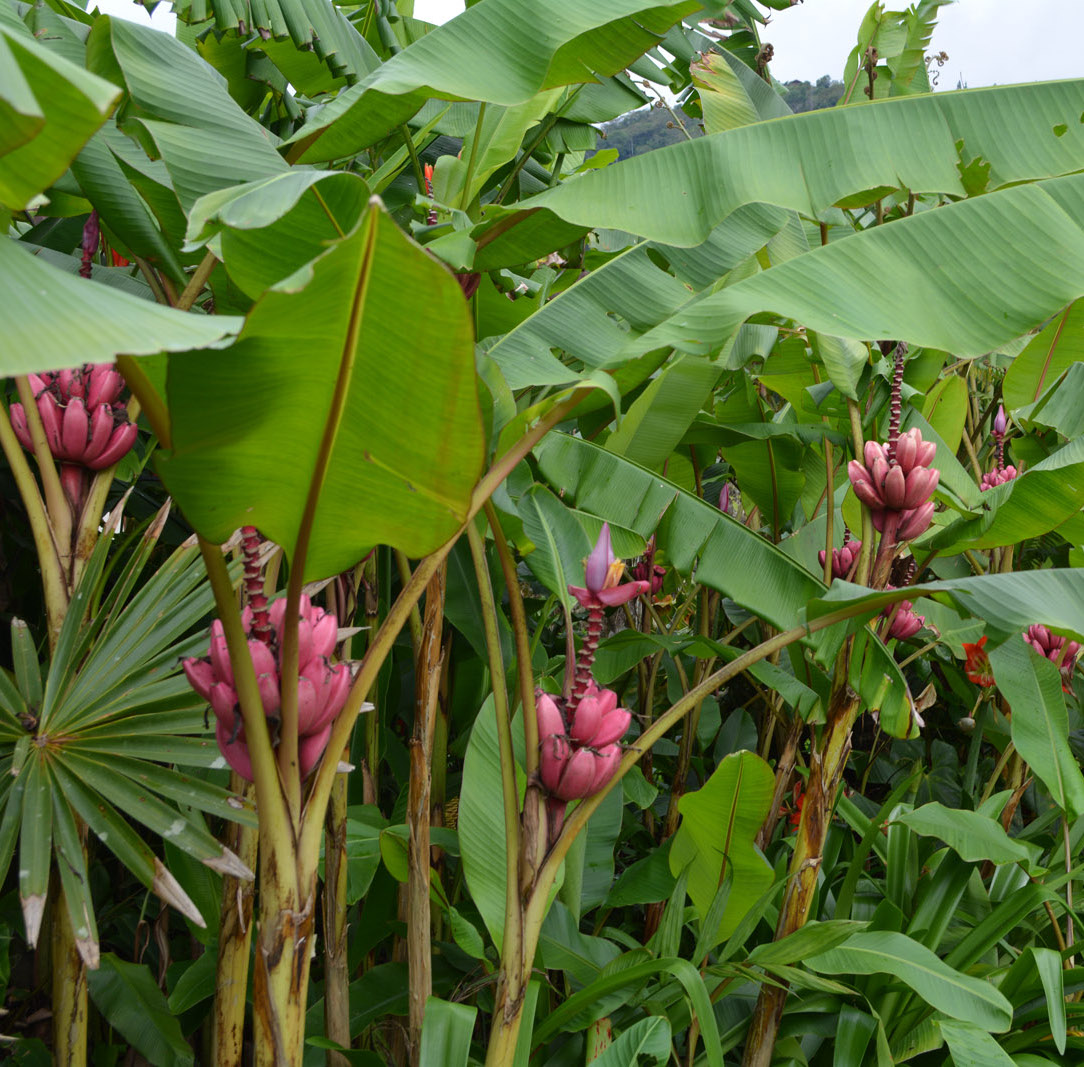
\includegraphics[scale=0.24]{redbanana3.jpg}
  \hspace{1cm}
%  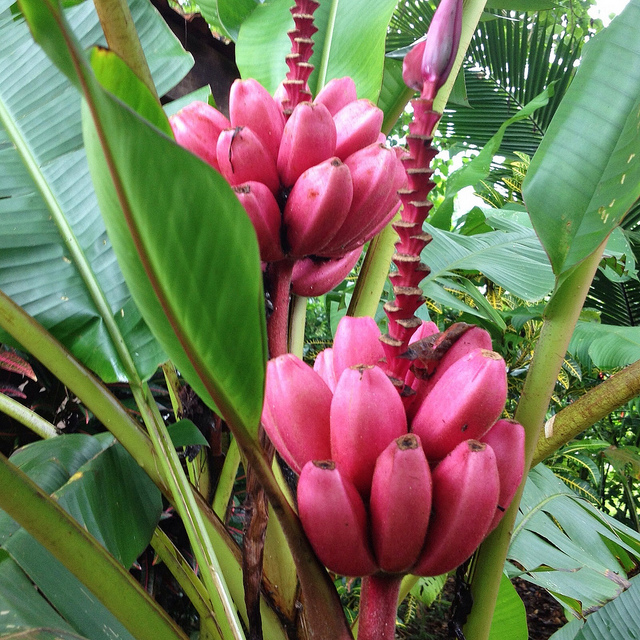
\includegraphics[scale=0.4]{redbanana1.jpg}
%  \hspace{1cm}
  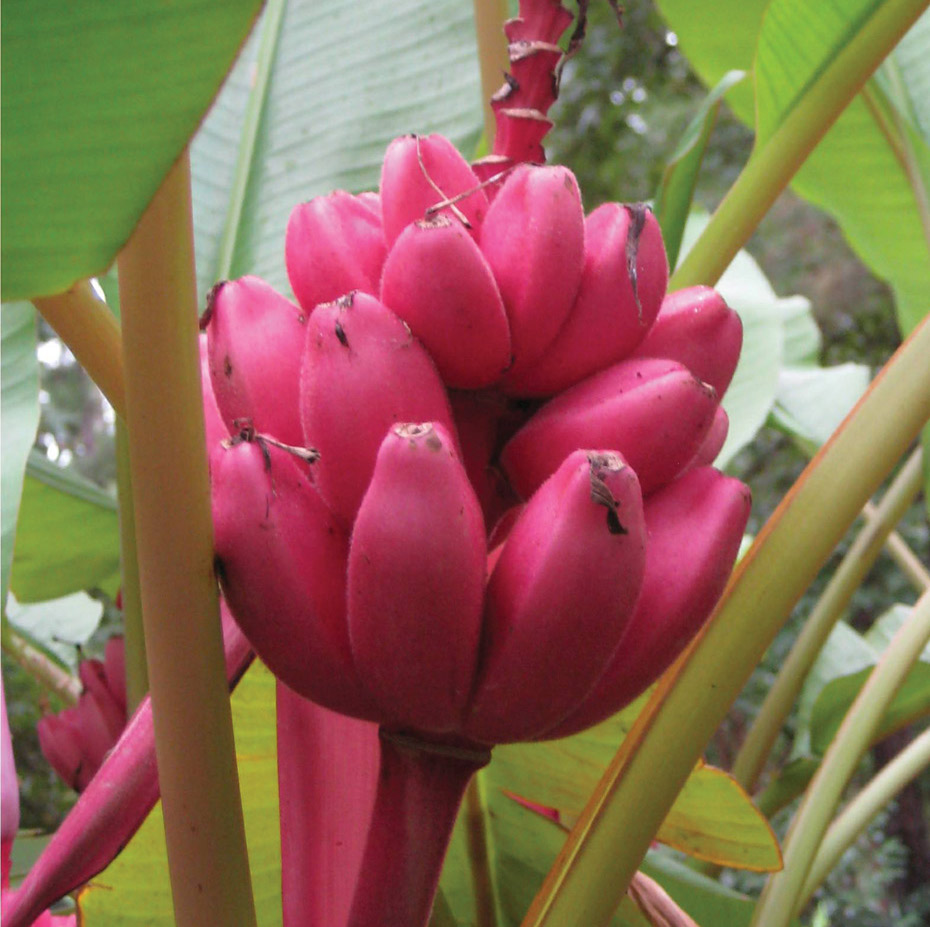
\includegraphics[scale=0.276]{redbanana2.jpg}
  \hspace{1cm}
  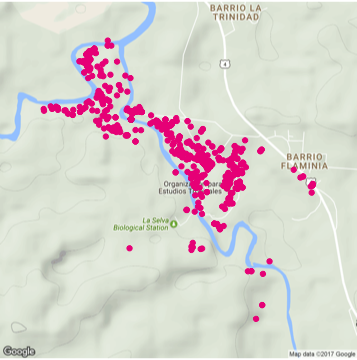
\includegraphics[scale=0.724]{Plot of redbanana.png}
  \vspace{0.5cm}
	
\end{block}
\vfill


%=============================================================%
\begin{block}{Epidemic-Type Aftershock Sequence (ETAS) Model}
%=============================================================%

\begin{itemize}
	\item The spatial-temporal ETAS model (Ogata, 1998) is a point process model where \red{the rate of an earthquake of magnitude-M occurring at time $t$ and location $(x,y)$ depends on the histroy of occurrences $H_t$}, characterized by	the conditional intensity function:
	      $$\lambda(t,x,y|H_t)=\mu(x,y)+\sum \limits_{\{i:t_i<t\}}\frac{K_0}{(t-t_i+c)^p} \cdot  \frac{e^{\alpha(M-M_0)}}{((x-x_i)^2+(y-y_i)^2+d)^q}$$
	      $\mu(x, y):$ A non-homogeneous background rate.\\
	      $\sum:$ Triggering function defined in the earthquake context.\\
	      $K_0,\alpha, c, p, d, q:$ Parameters to be estimated.
	\vspace{0.5cm}
  \item \red{The ETAS model for red banana plants} by Balderama (2012) is
        $$\displaystyle{\lambda(t,x,y|H_t)=(1-\rho)\mu(x,y)+\frac{\rho\alpha\beta}{\pi}\sum \limits_{\left\{i:t_i<t\right\}}e^{-\alpha(t-t_i)-\beta\left\{(x-x_i)^2+(y-y_i)^2\right\}}}$$
        $\frac{\balpha\bbeta}{\bpi}:$ A normalizing constant so that $\sum$ integrates to unity.\\
        $\balpha:$ Exponential decay rate due to \red{temporal distance apart}.\\
        $\bbeta:$ Exponential decay rate due to \red{spatial distance apart}.\\
        $\brho:$ \red{Proportion of events} attributed to triggering by other events.
  \vspace{0.4cm}
  \item The \red{log-likelihood function} for the occurrence of red banana plants is \\
   \hspace{1cm} $\displaystyle{logL=\sum \limits_{i=1}^{n}log\lambda(t_i,x_i,y_i)-\iint_A \int_0^\infty \lambda(t,x,y)dtdxdy}$  \\
   \hspace{3.1cm} $\displaystyle{=\sum \limits_{i=1}^{n}log\lambda(t_i,x_i,y_i)-(1-p)T\iint_A\mu(x,y)dxdy-pN}$
   
   
\end{itemize}
  


\end{block}
\vfill

}
\end{minipage}
\end{beamercolorbox}
\end{column}
%=============================================================%
\begin{column}{.33\textwidth}
\begin{beamercolorbox}[center,wd=\textwidth]{postercolumn}
\begin{minipage}[T]{.97\textwidth} % tweaks the width, makes a new \textwidth
\parbox[t][\columnheight]{\textwidth}{ % must be some better way to set the the height, width and textwidth simultaneously
% Since all columns are the same length, it is all nice and tidy.  You have to get the height empirically
%=============================================================%
%=============================================================%
%=============================================================%
%===================   SECOND COLUMN   =======================%
%=============================================================%
%=============================================================%
%=============================================================%



%=============================================================%
\begin{block}{Bayesian Estimation}
%=============================================================%

 	\begin{itemize}
		\item \textbf{Bayesian Analysis:} A statistical paradigm that answers research questions about unknown parameters using probability statements.
		\vspace{0.4cm}
		\item \textbf{Prior Distribution:} A probability distribution with respect to \red{current knowledge about parameters}, written as \boldmath{\red{$p(\theta)$}}.
		\vspace{0.4cm}
		\item \textbf{Likelihood:} \red{The information regarding parameters} contained by new data $y$, which is proportional to \red{$p(y|\theta)$}. 
		\vspace{0.4cm}
		\item \textbf{Posterior Distribution:} An updated probability distribution, on which all Bayesian inference is based, produced by \red{the combination of likelihood and the prior}, written as \red{$p(\theta|y)$}.
		\vspace{0.4cm}
		\item The posterior is proportional to the prior times the likelihood:\\ 
		\vspace{0.6cm}
		$\displaystyle{p(\theta|y)=\frac{p(\theta)p(y|\theta)}{\int p(\theta)p(y|\theta)d\theta}}$
		\ , where \red{$\theta = \{\alpha, \beta, \rho\}$}
	\end{itemize}


\end{block}
\vfill
%=============================================================%
\begin{block}{Results of Bayesian Estimation}
%=============================================================%
\vspace{0.3cm}
  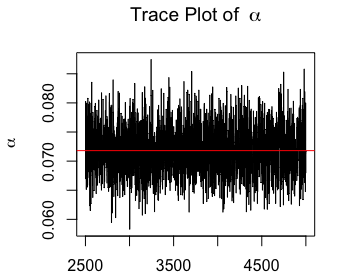
\includegraphics[scale=0.8]{TP of a.png}
  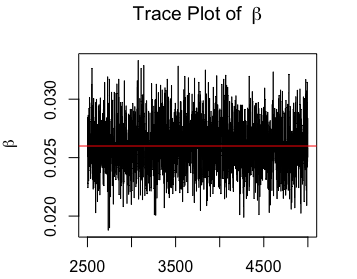
\includegraphics[scale=0.8]{TP of b.png}
  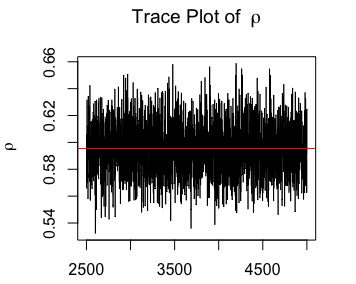
\includegraphics[scale=0.8]{TP of p.png}\\
  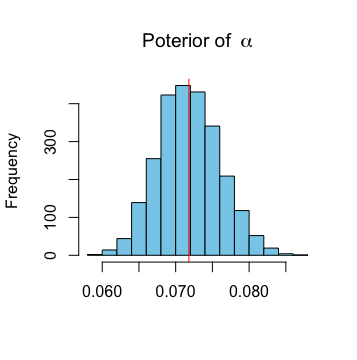
\includegraphics[scale=0.8]{P of a.png}
  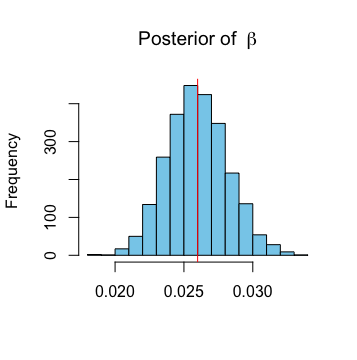
\includegraphics[scale=0.8]{P of b.png}
  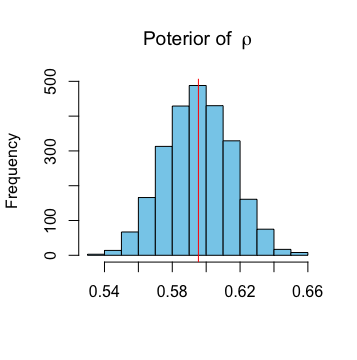
\includegraphics[scale=0.8]{P of p.png}

\vspace{-1.5cm}

 \renewcommand\arraystretch{1.3}
 \begin{center}
 \begin{tabular}{c|cc}
  %\hline
  \textbf{Parameter}  & \textbf{\blue{Posterior Mean}} & \textbf{Posterior SD} \\ \hline
  \large{$\balpha$}    & \blue{\large{0.0718}}  & \large{0.0042}  \\ %\hline
  \large{$\bbeta$}     & \blue{\large{0.0260}}  & \large{0.0022}  \\ %\hline
  \large{$\brho$}      & \blue{\large{0.5958}}  & \large{0.0195}  \\ %\hline
 \end{tabular}  
 \end{center}
 
 \begin{itemize}
  \item $\balpha$: The intensity of triggering events \red{decays at a rate of $1-e^{-0.0718}=6.93\%$ for every week that passes}.
  \vspace{0.3cm}
  \item $\bbeta$:  The intensity of triggering events \red{decays at a rate of $1-e^{-0.026}=2.57\%$ for every squared distance (in meters) away}.
  \vspace{0.3cm}
  \item $\brho$: \red{59.58\% of events were triggered} by previous events. Thus,\\
  \red{40.42\%  is the background rate}, i.e., percentage of immigrant events.
 \end{itemize}
 
\end{block}
\vfill

%========================================
\begin{block}{Bayesian Estimate Versus MLE}
%========================================

\red{Maximum Likelihood Estimates} obtained by Newton-Raphson algorithm:
  \begin{center}
  \renewcommand\arraystretch{1.3}
  \begin{tabular}{c|cc}
  %\hline
  \textbf{Parameter}  & \blue{\textbf{MLE}} & \textbf{Standard Error} \\ \hline
  \large{$\balpha$}    & \blue{\large{0.0761}}     & \large{0.0045} \\ %\hline
  \large{$\bbeta$}     & \blue{\large{0.0292}}     & \large{0.0022} \\ %\hline
  \large{$\brho$}      & \blue{\large{0.5767}}     & \large{0.0193} \\ %\hline
  \end{tabular}
  \end{center}
\begin{itemize}
  \item \green{Estimates from Bayesian MCMC are very close to MLEs.}
  \item \green{Bayesian estimates have such small standard deviations that can be considered as excellent estimates.}
  
\end{itemize}

\end{block}
\vfill
}

\end{minipage}
\end{beamercolorbox}
\end{column}
%=============================================================%
\begin{column}{.33\textwidth}
\begin{beamercolorbox}[center,wd=\textwidth]{postercolumn}
\begin{minipage}[T]{.97\textwidth}  % tweaks the width, makes a new \textwidth
\parbox[t][\columnheight]{\textwidth}{ % must be some better way to set the the height, width and textwidth simultaneously
% Since all columns are the same length, it is all nice and tidy.  You have to get the height empirically
%=============================================================%
%=============================================================%
%=============================================================%
%===================   THIRD COLUMN    =======================%
%=============================================================%
%=============================================================%
%=============================================================%


%=============================================================%
\begin{block}{Markov Chain Monte Carlo (MCMC Algorithm)}
%=============================================================%


	\begin{itemize}
			\item \textbf{Goal of MCMC:} Draw samples from a posterior distribution without having to know its exact height (probability) at any point.
%			\vspace{0.3cm}
%		\item \textbf{MCMC Algorithms:} A class of algorithms for \red{sampling from a probability distribution based on constructing a Markov Chain} that has the desired distribution as its stationary distribution. 
			\vspace{0.3cm}
		\item \textbf{Monte Carlo Methods:} A class of algorithms relies on repeated random sampling to obtain numerical results.
		\vspace{0.3cm}
 		\item \textbf{Markov Chain:} A type of Markov Process that has either discrete state space or discrete index set (often representing time).

			\begin{itemize}
	  	\item	The state of the chain after a number of steps is then used as a sample of the desired distribution.
%		  \item The quality of the sample improves as a function of the number of steps.
		  \end{itemize}
		  \vspace{0.2cm}
		  
	 
	  
%	  \begin{itemize}
%	    \item \textbf{Markov Process:} A process exhibits the Markov Property.
%	  	\item \textbf{Markov Property:} Given a process which is at a state $X_n$ at a particular point of time, the probability of $X_{n+1}=k$, where $k$ is any of the $M$ states the process can hop to, will only be dependent on which state it is at the given moment of time. And not on how it reached the current state. Mathematically speaking:
%		$$\displaystyle{P(X_{n+1}=k|X_n=k_n,X_{n-1}=k_{n-1},\ldots,X_1=k_1)=P(X_{n+1}=k|X_n=k_n)}$$
		  
%		\end{itemize}
		
		
		
		\item \textbf{MCMC Algorithm:}
		  \begin{enumerate}
	
    		\item Set up prior distributions and proposal distributions
    		\vspace{0.1cm}
    		  \renewcommand\arraystretch{1.3}
          \begin{center}
          \begin{tabular}{c|cc}
          \textbf{Parameter}  & \blue{\textbf{Prior Distribution}} & \textbf{Proposal Distribution}\\ \hline
          \large{$\balpha$}    & \blue{Gamma(1,10)}   & Normal($\balpha_0$,0.1)  \\ %\hline
          \large{$\bbeta$}     & \blue{Gamma(1,10)}   & Normal($\bbeta_0$,0.1)  \\ %\hline
          \large{$\brho$}      & \blue{Uniform(0,1)}  & Beta($\brho_0$,$1-\brho_0$)   \\ %\hline
          \end{tabular}  
         \end{center}
          
      \vspace{0.3cm}  
    		\item Initialize $\btheta$  by randomly picking a \red{initial state} from each prior.
    %		Start at a random initial state (randomly pick an initial number from the prior)
    		 
    		\item For $t$ in (1:50000), \red{update $\btheta$}:
    		 \begin{itemize}
	       \item \red{Propose a candidate $\balpha_1$} (randomly pick a candidate state from the proposal distribution based on current state $\balpha_0$).
	        \item Compute \red{Metropolis-Hastings ratio \textbf{R}}, which is \red{$\frac{p(\alpha_1|y)}{p(\alpha_0|y)}$}.
	        \item \red{Accept $\balpha_1$ and replace $\balpha_0$ at probability \textbf{R}}.
	        \item Proceed the same procedure above on $\bbeta$ and $\brho$.
	        \item \red{Record $\btheta$} after each iteration.
	       \end{itemize}
	       
	       \item After 50,000 iterations, return all states for parameters. \red{The 50,000 samples of each parameter make the posterior distributions}.
	       \item Compute \red{the means of samples} as the estimates of parameters.
	       \end{enumerate}
	      
		  
		\vspace{0.4cm}
		
		
		
		\item \textbf{Thinning:} \red{Discard all but $10^{th}$ observations} to get rid of autocorrelation to guarantee the independecy of samples.
		\vspace{0.4cm}
		\item \textbf{Burn-in:} \red{Throwing away first 2500 observations} to minimize the effect of initial values on the posterior inference.
		
	\end{itemize}
	

\end{block}
\vfill

%=============================================================%
\begin{block}{Future Work}
%=============================================================%


\begin{itemize}
\item \red{Simulation} needs to be done to check if the adjusted ETAS model fits the actual red banana plants data.
\vspace{0.4cm}
\item \red{More environment covirates and variables} should be considered into the spreading pattern of red banana plants, such as the distance from rivers, the amount of sunlight, elevation of plants etc.
\vspace{0.4cm}
\item The adjusted ETAS model needs to be \red{applied on other invasive speicies or point-process natural events} to assess its effectiveness.
\end{itemize}



\end{block}
\vfill

%=============================================================%
\begin{block}{Reference}
%=============================================================%

\begin{thebibliography}{}

\bibitem{Ogata}%just a name%
Ogata, Y.(1988),
``Statistical Models for Earthquake Occurrences and Residual Analysis for Point Processes,"
\textit{Journal of the American Statistical Association}, 83, 9-27.

\bibitem{Balderama}
Balderama, E.(2012),
``Spatial-Temporal Branching Point Process Models in the Study of Invasive Species,"
\textit{University of California, Los Angeles}

\end{thebibliography}


\end{block}
% \vfill
}
\end{minipage}
\end{beamercolorbox}
\end{column}
%%%%%%%%%%%%%%%%%%%%%%%%%%%%%%%%%%%%%%%%%%%%%%%
%%%%%%%%%%%%%%%%%%%%%%%%%%%%%%%%%%%%%%%%%%%%%%%












%++++++++++++++++++++++++++++++++++++++++++++++++++++++++++++++%
%++++++++++++++++++++++++++++++++++++++++++++++++++++++++++++++%
%++++++++++++++++++++++++++++++++++++++++++++++++++++++++++++++%
%++++++++++++++++++++++++++++++++++++++++++++++++++++++++++++++%
%++++++++++++++++++++++++++++++++++++++++++++++++++++++++++++++%
%++++++++++++++++++++++++++++++++++++++++++++++++++++++++++++++%
% end the columns
  \end{columns}
  \vskip1ex
  %\tiny\hfill\textcolor{ta2gray}{Created with \LaTeX \texttt{beamerposter}  \url{http://www-i6.informatik.rwth-aachen.de/~dreuw/latexbeamerposter.php}}

  %\tiny\hfill{Created with \LaTeX \texttt{beamerposter}
  %\url{http://www4.ncsu.edu/$\sim$dmvock/} \hskip1em}
\end{frame}
}
\end{document}


%%%%%%%%%%%%%%%%%%%%%%%%%%%%%%%%%%%%%%%%%%%%%%%%%%%%%%%%%%%%%%%%%%%%%%%%%%%%%%%%%%%%%%%%%%%%%%%%%%%%
%%% Local Variables:
%%% mode: latex
%%% TeX-PDF-mode: t
%%% End:
